\section{Fehlerbehandlungen}
Fehlerbehandlungen stehen der Performance eines Programms ständig im Weg, dies ist auch Logisch
zu erklären, da abgefangen und überprüft werden muss, ob es zu einem Fehler kam. Dafür muss
Programmcode hinzugefügt werden, der nicht essentiell für den eigentlichen Ablauf des Programms
ist. Dennoch kommt der Programmierer nicht drum herum Fehlerbehandlungen in seinem System zu
integrieren, da es immer zu unvorhergesehenen Fehlern kommen kann.

\subsection{Exceptions}
Um einen Fehler zu behandeln, kann der Programmierer einen Status Code zurückgeben und diesen
Überprüfen oder eine \emph{Exception} werfen und die Funktion die Potentiell eine
\emph{Exception} werfen könnte mit einem \emph{Try-Catch} Block umringen. Die Vorteile von
\emph{Exceptions} gegenüber von Status Codes, sind in dem folgenden Zitat schön zusammengefasst:

\begin{zitat}
    The use of exceptions isolates the error handling code from the normal flow of program
    execution, and unlike the error code approach, it cannot be ignored or forgotten. Also,
    automatic destruction of stack objects when an exception is thrown renders a program less likely to leak
    memory or other resources. With exceptions, once a problem is identified, it cannot be ignored –
    failure to catch and handle an exception results in program termination \cite{TechnicalReport}.
\end{zitat}

Wie zu sehen ist, bieten \emph{Excetions} nennenswerte Vorteile und haben somit auch eine
Daseinsberechtigung.
\newline
\newline
Obwohl klare Vorteile existieren, sind \emph{Exceptions} seit ihrer Einführung ein stark
umstrittenes Thema. Dies hat sich auch nach der Tabellen orientierten Optimierung, dass kein
Performance Verlust entsteht, wenn keine \emph{Exceptions} geworfen wird, nicht geändert. Der
Grund für die Umstrittenheit ist, dass \emph{Exceptions} gegen das \emph{zero-overhead prinzip}
verstoßen. Auch bei der Betrachtung der Performance eines Programms zeigen sich \emph{Exceptions}
als sehr Problematisch, da diese Dynamisch zur Laufzeit, zum Beispiel auf dem \emph{Heap}
erstellt werden müssen, was wie im Kapitel Speicher Management gezeigt, schon sehr teuer ist, und
anschließend noch der Dynamische Type der \emph{Exceptions} herausgefunden werden muss, was in
einem \emph{$dynamic\_cast$} resultiert. Ein weiteres Problem, welches mit der Verwendung von
\emph{Exceptions} kommt, ist dass nicht gesagt werden kann, wie lange es braucht bis eine
\emph{Exceptions} vollständig abgearbeitet ist. Dadurch kann die Situation entstehen, dass
während eine \emph{Exceptions} verarbeitet wird, eine andere geworfen wird und somit auch eine
unbestimmbare menge an Speicher gebraucht wird.\cite{HandsOn}

\subsection{Expected}
\emph{Exceptions} sind zwar sehr langsam, jedoch bringen sie wie vorher im Unterkapitel
\emph{Exceptions} erwähnt auch nennenswerte Vorteile gegenüber einfachen Status Codes. Deswegen
kann auf die Alternative von \emph{Expected} zurückgegriffen werden, welches einen Kompromiss
zwischen Status Codes und \emph{Exceptions} darstellt. \emph{Expected} wird durch
\emph{Templateklasse} repräsentiert, die Beispielhaft als Pseudocode, wie folgt aussehen könnte:

\begin{lstlisting}[
    caption={Pseudocode einer Expected Klass\cite{OverheadExceptions}},
    label=lst:Expected-Klasse,
    language=C++,frame=tlrb]
  				
template <class T>
class Expected {
private:
    union {
        T value;
        std::exception_ptr exception;
    };
public:
    Expected(const T& value) { ... }
    
    Expected(const std::exception_ptr& e) { ... }
    
    bool hasError() { ... }
    
    T getValue() { ... }
    
    std::exception_ptr getException() { ... }
};
\end{lstlisting}

Wie zu sehen ist, sind die zwei Variablen in einem \emph{union} gespeichert um das \emph{zero
overhead prinzip} nicht zu verletzen. Die Idee dahinter ist es, die \emph{Exception} nicht mehr
zu werfen, sondern diese wie einen erwarteten Wert zurück zu geben. Sollte die Funktion
erfolgreich durchlaufen, dann kann der erwartete Wert mittels der Funktion \emph{getValue()}
bekommen werden. Sobald jedoch ein Fehler aufkommt, wird dieser in der gleichen \emph{Instance}
gespeichert und mittels \emph{hasError()} kann dann überprüft werden, ob ein Fehler vorliegt.
Dadurch wurde erreicht, dass noch Metainformationen, zum Beispiel repräsentiert anhand von einem
\emph{String}, im Falle eines Fehlers zurückgegeben werden kann \cite{OverheadExceptions}[vgl.].
\newline

\begin{figure}[h]
    \centering
    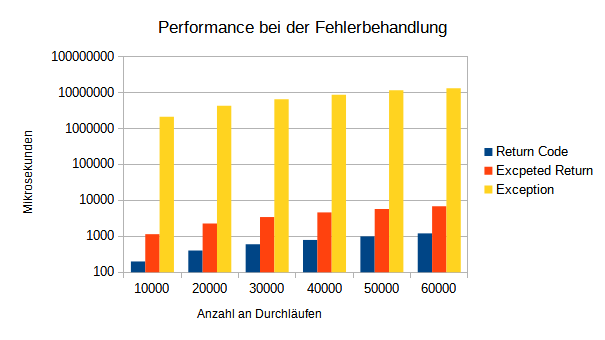
\includegraphics[width=0.5\textwidth]{bilder/Performance_Fehlerbehandlung}
    \caption[Fehlerbehandlung]{Performance bei der Fehlerbehandlung}
    \label{img:fehlerbehandlung}
\end{figure}

Abbildung \ref{img:fehlerbehandlung} zeigt den Performance unterschied zwischen der vorig
besprochenen \emph{Expected} Klasse als \emph{return} Wert und einen \emph{int} als \emph{return}
Wert, sowie der Fall, dass eine \emph{Exception} geworfen wird. Klar zu erkennen ist zwar dass
der Status Code immer noch wesentlich Performanter ist, jedoch ist der Unterschied zu
\emph{Exceptions} deutlich geringer.

\subsection{Zusammenfassung}
Trotz dessen, dass \emph{Exceptions} klare Vorteile bieten und durch Optimierungen, die
Performance nicht verschlechtern, wenn diese nicht geworfen werden, ist der Verlust an
Performance zu enorm, wenn diese geworfen werden. Große Firmen wie zum Beispiel Google haben
\emph{Exceptions} sogar komplett aus Ihren Projekten verboten. Durch die \emph{Templateklasse}
\emph{Expected} existiert eine lukrative Alternative, die wesentlich Performanter ist als
\emph{Exceptions}. Dennoch, wenn das Maximum an Performance in einem Programm herausgeholt werden
soll, dann sollte mit Status Codes gearbeitet werden.